\documentclass{beamer}
\usetheme{Madrid}
\usecolortheme{default}
\usepackage{graphicx}
\usepackage{booktabs}
\usepackage{amsmath}
\usepackage{CJK}
\usepackage{CJKutf8}

\begin{document}
\begin{CJK*}{UTF8}{gbsn}%{bsmi}

\begin{frame}[plain]
    \centering
    
\includegraphics[width=\linewidth]{Figures/IALP2025.png}
    \vspace{1.0cm}

    {\Large \textbf{Quantitative Evaluation of Translation Quality and Computational Efficiency}}\\[0.4em]
    {\Large in Semantic vs. Phonetic Strategies for Chinese Scientific Terms}\\[1.0em]

    \textbf{Li Weigang}\inst{1}, \textbf{Pedro Carvalho Brom}\inst{2}, \textbf{Rafael Marconi Ramos}\inst{1}\\
    \inst{1} Department of Computer Science, University of Brasília\\
    \inst{2} Department of Mathematics, Federal Institute of Brasília\\[1.2em]

    %\textit{IALP 2025 -- International Conference on Asian Language Processing}\\
    \textit{Kuching, Malaysia -- August 2025}
\end{frame}

\begin{frame}{Motivation}
\begin{itemize}
    \item Chinese scientific terminology translation includes semantic and phonetic strategies.
    \item Phonetic transliteration often results in unintelligible compound names.
    \item Need for systematic evaluation of translation quality and efficiency.
    \item Rise of LLMs (Grok, GPT, DeepSeek) offers new tools for analysis.
\end{itemize}

\end{frame}

%-------------------------------
\begin{frame}{Advantages of Chinese Periodic Table - 中文元素周期表优势}
Unlike phonetic languages (e.g., English, Portuguese), where chemical element names average 7.82 letters (max 13, e.g., Rutherfordium), Chinese uses a single character per element (e.g., “氢” for hydrogen), encoded in 3 bytes via Unicode/UTF-8. This compactness, rooted in the pictophonetic structure from “Shuowen Jiezi-说文解字” (c. 100 AD), integrates semantic richness—e.g., “氢” implies gaseous lightness—outperforming Japanese (13.73 bytes) and Korean (8.97 bytes) transliterations.
\begin{figure}
    \centering
    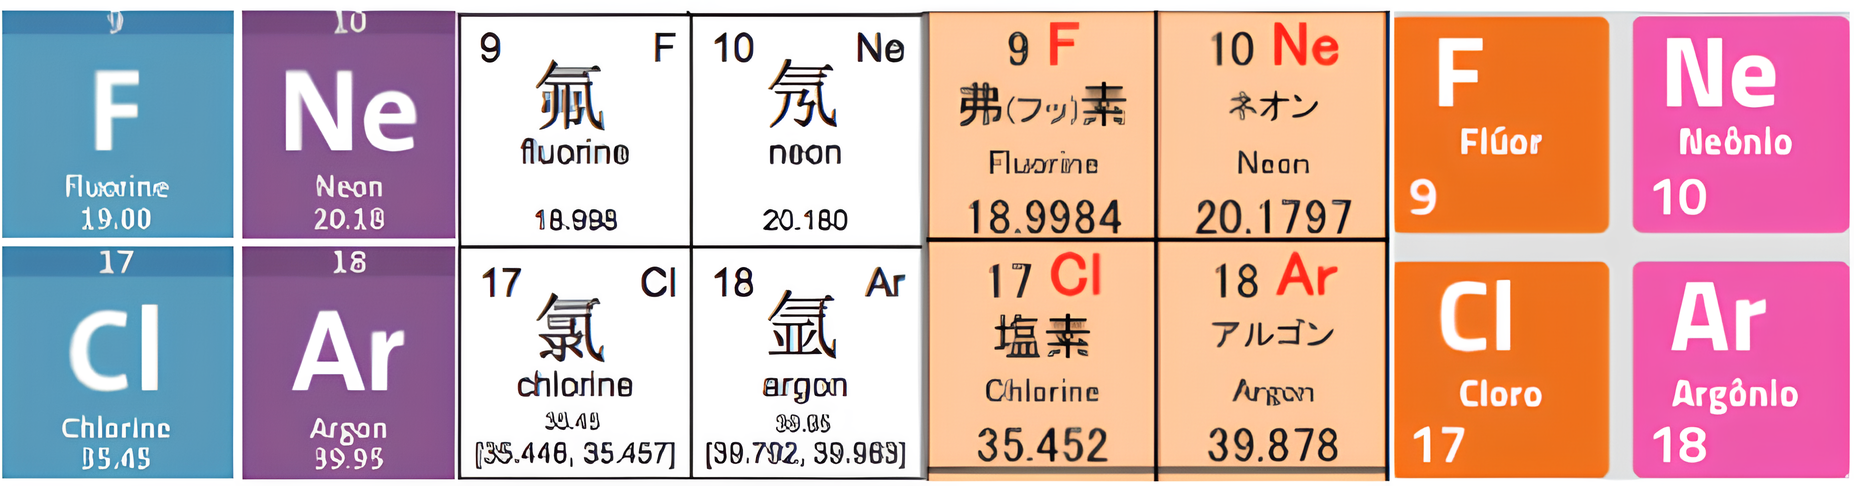
\includegraphics[width=0.8\linewidth]{img/Four elements 2.png}
    \caption{Examples of four elements (fluorine, neon, chlorine, and argon) from the periodic tables of English, Chinese, Japanese, and Portuguese.}
\end{figure}

\end{frame}

%-------------------------------
\begin{frame}{Research Questions}
\begin{itemize}
    \item How do semantic and phonetic strategies perform in scientific translation?
    \item Can back-translation powered by LLM (LLM-BT) reliably assess translation fidelity?
    \item What are the computational costs of different strategies?
    \item Do LLMs outperform traditional tools in complex term translation?
\end{itemize}
\end{frame}

%-------------------------------
\begin{frame}{LLM-BT Framework}
\begin{figure}
    \centering
    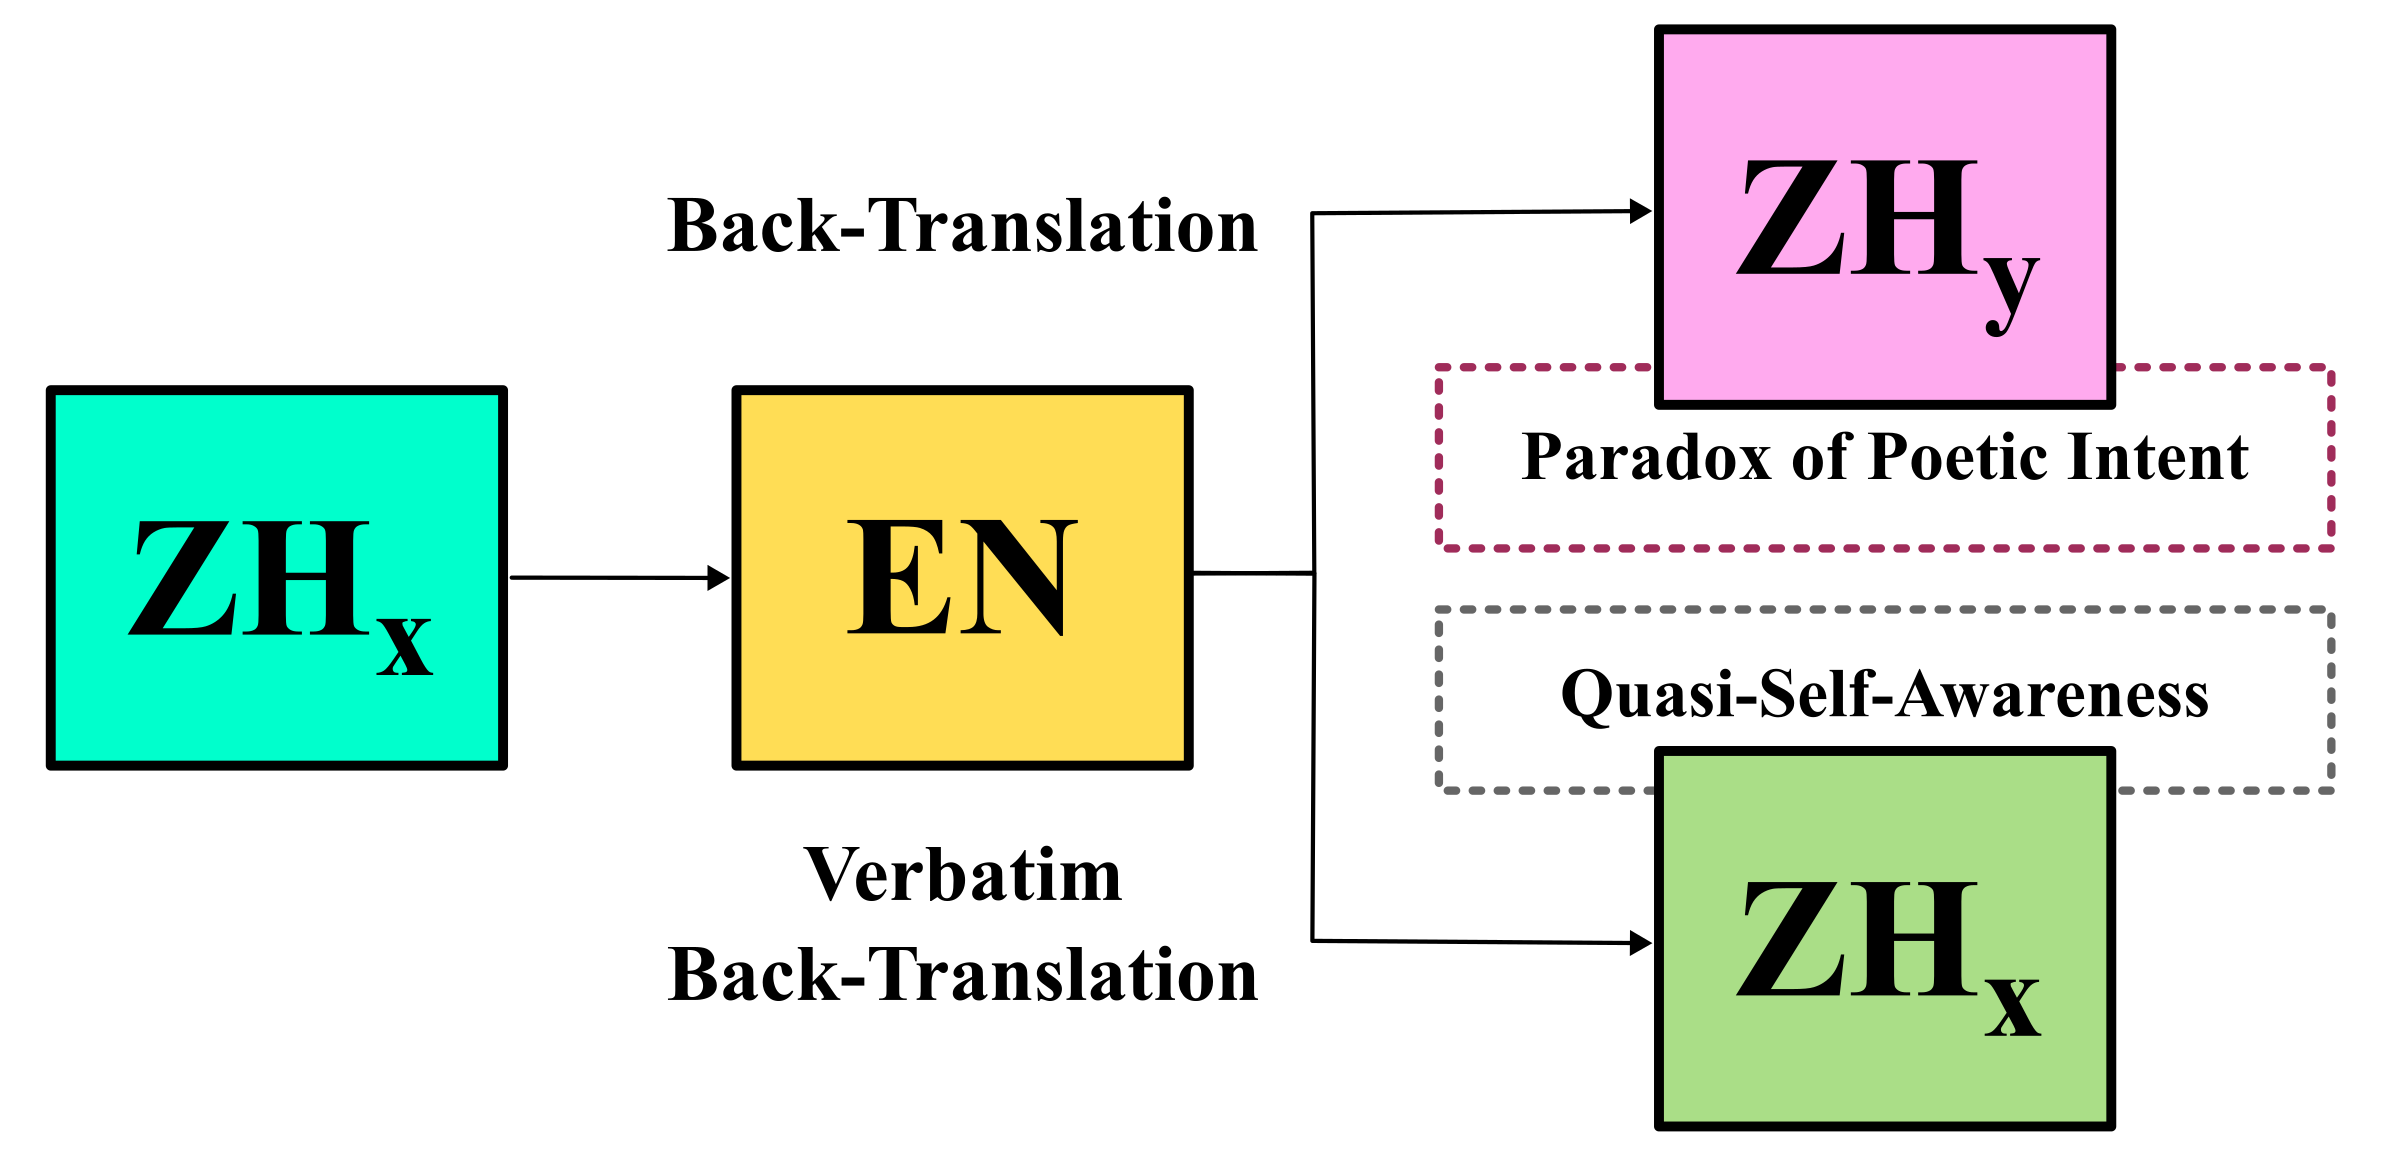
\includegraphics[width=0.8\linewidth]{Figures/bt-flowchart.png}
    \caption{Conceptual Diagram: LLM-Back-Translation Workflow: Chinese $\rightarrow$ English $\rightarrow$ Chinese. The Paradox of Poetic Intent (诗意意境悖论) in back-translation vs. emergent Quasi-Self-Awareness (类自觉性) in LLM verbatim back-translation, where $ZHx$ is the original Chinese text, $EN$ is the translated English text and $ZHy$ is the back-translated Chinese text.}
\end{figure}
\end{frame}

%-------------------------------
\begin{frame}{Datasets}
\begin{itemize}
    \item \textbf{PT-ZH118}: Periodic table in six languages including Chinese with pictophonetic and semantic translation.
    \item \textbf{HO-ZH58}: 58 heterocyclic compounds (phonetic transliteration - 杂环化合物以音译命名).
    \item \textbf{XDJ's Corpus}: Xue Dejiong’s statements on terminology challenges （薛德炯困境）. This text poses unique linguistic challenges, blending technical, cultural, and rhetorical elements, making it an ideal benchmark for evaluating machine translation performance.
\end{itemize}
\end{frame}

%-------------------------------
\begin{frame}{Computational Cost Analysis}
\begin{block}{Equation - 与英文字节表达比}
The ratio $\gamma$ (gamma) compares element or compound nomenclature in a given language to English. If the representation number is the number of bytes $N_{L,\text{byte}}$, then $\gamma$ is the byte ratio relative to English:
\[
\gamma_\text{byte} = \frac{N_{L,\text{byte}}}{N_{\text{Eng},\text{byte}}}
\]
\end{block}
\begin{itemize}
    \item Chinese element names: 3 bytes vs. English 7.82 → $\gamma = 0.38$
    \item Japanese element names: 13.73 bytes → $\gamma = 1.76$
    \item Phonetic transliteration increases byte cost
\end{itemize}
\end{frame}

%-------------------------------
\begin{frame}{Semantic strategy}

\begin{table*}%[h!]
\centering
\caption{Comparison of Representation Indicators for Periodic Table Names in Several Languages}
\begin{tabular}{ccccc}
\hline
\textbf{Languages} & \textbf{Min letters} & \textbf{Max letters} & \textbf{Ave letters} & \textbf{Ave bytes}  \\ 
\textbf{语言} & \textbf{最少字符} & \textbf{最多字符} & \textbf{平均字符} & \textbf{平均字节} \\ \hline
\textbf{English} & 3 & 13 & 7.82 & 7.82 \\ 
\textbf{Latin} & 4 & 13 & 8.07 & 8.07 \\ 
\textbf{Portuguese} & 4 & 12 & 7.05 & 7.27  \\ 
\textbf{Russian} & 3 & 11 & 6.66 & 13.32  \\ 
\textbf{Japanese} & 1 & 9 & 4.58 & 13.73  \\ 
\textbf{Korean} & 1 & 8 & 2.99 & 8.97  \\ 
\textbf{Chinese} & 1 & 1 & 1 & 3  \\ \hline
%\textbf{SWPC} & 4 & 8 & 4.75 & 4.75 & 0.61 \\ \hline
\end{tabular}
\label{tab:letter_byte_comparison}
\end{table*}
\end{frame}

%-------------------------------
\begin{frame}{Phonetic Strategy}
Comparison of Representation Indicators for Phonetically Transcribed Organic Compound Names
\begin{table*}%[htbp]
\centering
\label{tab:comparison}
\begin{tabular}{ccccc}
\hline
\textbf{Language} & \textbf{Min letters} & \textbf{Max letters} & \textbf{Ave letters} & \textbf{Ave bytes}  \\
\textbf{语言} & \textbf{最少字符} & \textbf{最多字符} & \textbf{平均字符} & \textbf{平均字节}  \\
\hline
English & 9 & 35 & 13.67 & 13.67 \\

Japanese & 4 & 18 & 6.43 & 19.34  \\

Korean & 2 & 17 & 5.05 & 15.16  \\

Chinese & 3 & 12 & 6 & 18  \\
\hline
\end{tabular}
\end{table*}
\end{frame}

%-------------------------------
\begin{frame}{LLM-BT performance validation}

We employ a back-translation method to translate “Xue Dejiong’s Dilemma." Two main categories of models are selected: (a) widely used translation tools such as Google Translate, Baidu Translate, and Sogou Translate; and (b) large language models (LLMs) including ChatGPT, Grok, DeepSeek, and Gemini. These publicly accessible systems allow any user to replicate the computations.

采用回译法翻译《薛德炯的困境》。主要选取两类模型：（a）广泛使用的翻译工具，例如谷歌翻译、百度翻译和搜狗翻译；（b）大型语言模型（LLM），包括 ChatGPT、Grok、DeepSeek 和 Gemini。这些公开的系统允许任何用户复制计算。

\end{frame}

\begin{frame}{Corpus of “Xue Dejiong’s Dilemma."}
\begin{itemize}
    
\item 《薛德炯的困境》原文片段: \textbf{  ``满纸咿哑, 一若番书, 虽有谪仙李太白其人, 恐亦难于索解。}'' 

\item “XDJ’s Dilemma." English translation by Grok: filling the page with gibberish, as if it were a foreign text. Even someone as extraordinary as the banished immortal Li Taibai (Li Bai) would likely find it difficult to decipher.

\item “XDJ’s Dilemma." back-translation to Chinese by Grok: \textbf{\begin{CJK*}{UTF8}{gbsn}满纸都是胡言乱语, 仿佛外文书籍。即使有谪仙李太白（李白）这样杰出的人物, 恐怕也难以理解。\end{CJK*}}
 
\end{itemize}
\end{frame}

%-------------------------------
%-------------------------------
\begin{frame}{Translation Quality Evaluation (BLEU)}
\begin{itemize}
    \item Back-translation (BT) used to assess fidelity: Chinese → English → Chinese
    \item BLEU score between original term and BT result
    \item Results from GPT-4, Grok, DeepSeek, GPT-4.5, etc.
\end{itemize}

\vspace{0.4cm}
\begin{block}{Observation}
    Semantic terms achieve BLEU $\approx$ 1.00; phonetic terms drop to BLEU $\approx$ 0.55–0.65.
\end{block}
\end{frame}

%-------------------------------

\begin{frame}{LLM-BT performance validation}
\begin{table}[h]
\centering
\caption{Comparison of BLEU Scores Across Two Rounds for XDJ’s Dilemma corpus} %for Different Translation Tools}
\label{tab:bleu_comparison}
\begin{tabular}{lccc}
\toprule
\textbf{LLM/Tool}         & \textbf{BLEU 1 (R 1)} & \textbf{BLEU 2 (R 2)} & \textbf{Change} \\
\midrule
Grok (xAI)               & 0.65                     & 0.61                     & -0.04          \\
DeepSeek V3              & 0.64                     & 0.58                     & -0.06          \\
ChatGPT 4.5              & 0.59                     & 0.59                        & 0              \\
ChatGPT 4                & 0.47                     & 0.50                     & +0.03          \\
Gemini Flash 2.0         & 0.51                        & 0.52                     & +0.01              \\
Google Translation       & 0.33                     & 0.44                     & +0.11          \\
Baidu Translation        & 0.25                     & 0.36                     & +0.11          \\
Mistral                  & 0.24                     & 0.46                     & +0.22          \\
Sogou Translation        & 0.17                     & 0.31                     & +0.14          \\
\bottomrule
\end{tabular}
\end{table}
\end{frame}



\begin{frame}{Example: Semantic vs. Phonetic LLM Back-Translation}
\begin{itemize}
    \item LLM-BT: Chinese → English → Chinese
    \item \textbf{Semantic}: 碳 → carbon → 碳 （BLEU = 1.00）
    \item \textbf{Phonetic}: 苯并噻唑 → benzothiazole → 苯硫唑? （$BLEU < 0.65$）
    \item \textbf{Observation}: LLMs struggle to reverse phonetic transliterations
\end{itemize}
\end{frame}

%-------------------------------
\begin{frame}{Cross-Language Comparison (BLEU)}
\begin{itemize}
    \item BLEU tested across Chinese, Japanese, Russian, Portuguese, etc. 
    \item Semantic translations consistently yield higher BLEU
    \item Using English → Chinese CN → Chinese TW → English to determine the scientific terminology
\end{itemize}

\vspace{0.4cm}
\begin{block}{Conclusion}
    Semantic strategy is more reversible and LLM-friendly across languages
\end{block}
\end{frame}

%-------------------------------
\begin{frame}{Findings and Insights}
\begin{itemize}
    \item Phonetic translations are not reliably reversible by LLMs
    \item BLEU favors literal fidelity, but BLEU $\approx$ 1.00 only in semantic cases
    \item Verbatim bias in LLMs causes false positives in translation confidence
    \item LLM output is influenced by instruction clarity and token noise
\end{itemize}
\end{frame}

%-------------------------------
\begin{frame}{Conclusion and Future Work}
\begin{itemize}
    \item LLM-BT offers a lightweight, scalable method for evaluating scientific terminology translation
    \item Strong evidence supports semantic over phonetic translation strategies
    \item Future work: integrate LLM evaluation into domain-specific NMT pipelines
    \item Broader implication: LLMs as evaluators, not just generators
\end{itemize}
\end{frame}

%-------------------------------
\begin{frame}{More reading}
\begin{itemize}
    \item The Paradox of Poetic Intent in Back-Translation: Evaluating the Quality of Large Language Models in Chinese Translation - https://arxiv.org/abs/2504.16286
    \item LLM-BT-Terms: Back-Translation as a Framework for Terminology Standardization and Dynamic Semantic Embedding - https://arxiv.org/abs/2506.08174

\end{itemize}
\end{frame}

%-------------------------------
\begin{frame}{Acknowledgments \& Q\&A}
\begin{itemize}
    \item GPT-4, Grok, DeepSeek used via NLPMetrics platform
    \item Special thanks to TransLab of UnB, Pedro Brom, Rafael Ramos
    \item Questions and discussion welcome!
\end{itemize}
\vspace{0.5cm}
\centering
\textit{Contact: \underline{weigang@unb.br}}
\end{frame}

\end{CJK*}
\end{document}
